\documentclass[a4paper]{book}
\usepackage{makeidx}
\usepackage{graphicx}
\usepackage{multicol}
\usepackage{float}
\usepackage{listings}
\usepackage{color}
\usepackage{ifthen}
\usepackage[table]{xcolor}
\usepackage{textcomp}
\usepackage{alltt}
\usepackage{ifpdf}
\ifpdf
\usepackage[pdftex,
            pagebackref=true,
            colorlinks=true,
            linkcolor=blue,
            unicode
           ]{hyperref}
\else
\usepackage[ps2pdf,
            pagebackref=true,
            colorlinks=true,
            linkcolor=blue,
            unicode
           ]{hyperref}
\usepackage{pspicture}
\fi
\usepackage[utf8]{inputenc}
\usepackage{mathptmx}
\usepackage[scaled=.90]{helvet}
\usepackage{courier}
\usepackage{sectsty}
\usepackage[titles]{tocloft}
\usepackage{doxygen}
\lstset{language=C++,inputencoding=utf8,basicstyle=\footnotesize,breaklines=true,breakatwhitespace=true,tabsize=8,numbers=left }
\makeindex
\setcounter{tocdepth}{3}
\renewcommand{\footrulewidth}{0.4pt}
\renewcommand{\familydefault}{\sfdefault}
\begin{document}
\hypersetup{pageanchor=false}
\begin{titlepage}
\vspace*{7cm}
\begin{center}
{\Large GSoC2011SfM \\[1ex]\large 0.1 }\\
\vspace*{1cm}
{\large Generated by Doxygen 1.7.4}\\
\vspace*{0.5cm}
{\small Sat May 28 2011 17:05:41}\\
\end{center}
\end{titlepage}
\clearemptydoublepage
\pagenumbering{roman}
\tableofcontents
\clearemptydoublepage
\pagenumbering{arabic}
\hypersetup{pageanchor=true}
\chapter{Class Index}
\section{Class Hierarchy}
This inheritance list is sorted roughly, but not completely, alphabetically:\begin{DoxyCompactList}
\item \contentsline{section}{OpencvSfM::Camera}{\pageref{class_opencv_sf_m_1_1_camera}}{}
\item \contentsline{section}{OpencvSfM::ExternPosEstim}{\pageref{class_opencv_sf_m_1_1_extern_pos_estim}}{}
\item \contentsline{section}{OpencvSfM::FieldOfView}{\pageref{class_opencv_sf_m_1_1_field_of_view}}{}
\item \contentsline{section}{OpencvSfM::MotionProcessor}{\pageref{class_opencv_sf_m_1_1_motion_processor}}{}
\item \contentsline{section}{OpencvSfM::Points3DEstim}{\pageref{class_opencv_sf_m_1_1_points3_d_estim}}{}
\item \contentsline{section}{OpencvSfM::PointsMatcher}{\pageref{class_opencv_sf_m_1_1_points_matcher}}{}
\item \contentsline{section}{OpencvSfM::PointsToTrack}{\pageref{class_opencv_sf_m_1_1_points_to_track}}{}
\begin{DoxyCompactList}
\item \contentsline{section}{OpencvSfM::PointsToTrackWithImage}{\pageref{class_opencv_sf_m_1_1_points_to_track_with_image}}{}
\end{DoxyCompactList}
\end{DoxyCompactList}

\chapter{Class Index}
\section{Class List}
Here are the classes, structs, unions and interfaces with brief descriptions:\begin{DoxyCompactList}
\item\contentsline{section}{\hyperlink{class_opencv_sf_m_1_1_camera}{OpencvSfM::Camera} (We will need this class, but \hyperlink{class_opencv_sf_m_1_1_point_of_view}{PointOfView} need our class too.. )}{\pageref{class_opencv_sf_m_1_1_camera}}{}
\item\contentsline{section}{\hyperlink{class_opencv_sf_m_1_1_camera_pinhole}{OpencvSfM::CameraPinhole} (This class represent the physical device which take the pictures. It is not related to a 3D position which is the role of the \hyperlink{class_opencv_sf_m_1_1_point_of_view}{PointOfView} class. The role of the class is to store only intra parameters (without radial distortion) )}{\pageref{class_opencv_sf_m_1_1_camera_pinhole}}{}
\item\contentsline{section}{\hyperlink{class_opencv_sf_m_1_1_camera_pinhole_distor}{OpencvSfM::CameraPinholeDistor} (This class represent the physical device which take the pictures. It is not related to a 3D position which is the role of the \hyperlink{class_opencv_sf_m_1_1_point_of_view}{PointOfView} class. The role of the class is to store intra parameters and radial distortion )}{\pageref{class_opencv_sf_m_1_1_camera_pinhole_distor}}{}
\item\contentsline{section}{\hyperlink{class_opencv_sf_m_1_1_motion_estimator}{OpencvSfM::MotionEstimator} }{\pageref{class_opencv_sf_m_1_1_motion_estimator}}{}
\item\contentsline{section}{\hyperlink{class_opencv_sf_m_1_1_motion_processor}{OpencvSfM::MotionProcessor} (This class try to create a commun interface for files loading. Indeed, if you want to use webcam, avi file of list of files, you will have to do some annoying processing, like iterate the different files of the directory. With \hyperlink{class_opencv_sf_m_1_1_motion_processor}{MotionProcessor}, you can now use a folder of image the same way you use a webcam or a video file )}{\pageref{class_opencv_sf_m_1_1_motion_processor}}{}
\item\contentsline{section}{\hyperlink{class_opencv_sf_m_1_1_point_of_view}{OpencvSfM::PointOfView} (This class represent the 3D position of the device which take the pictures. The role of the class is to store everything related to the filed of view: picture, 3D position, points, matches and 3D points )}{\pageref{class_opencv_sf_m_1_1_point_of_view}}{}
\item\contentsline{section}{\hyperlink{class_opencv_sf_m_1_1_points3_d_estim}{OpencvSfM::Points3DEstim} }{\pageref{class_opencv_sf_m_1_1_points3_d_estim}}{}
\item\contentsline{section}{\hyperlink{class_opencv_sf_m_1_1_points_matcher}{OpencvSfM::PointsMatcher} (A class used for matching descriptors that can be described as vectors in a finite-\/dimensional space )}{\pageref{class_opencv_sf_m_1_1_points_matcher}}{}
\item\contentsline{section}{\hyperlink{class_opencv_sf_m_1_1_points_to_track}{OpencvSfM::PointsToTrack} (This class can be used to store informations about points and features. This is an abstract class: you can't use it directly. Use for instance \hyperlink{class_opencv_sf_m_1_1_points_to_track_with_image}{PointsToTrackWithImage} )}{\pageref{class_opencv_sf_m_1_1_points_to_track}}{}
\item\contentsline{section}{\hyperlink{class_opencv_sf_m_1_1_points_to_track_with_image}{OpencvSfM::PointsToTrackWithImage} (This class can be used to find points and features in pictures using SIFT detector )}{\pageref{class_opencv_sf_m_1_1_points_to_track_with_image}}{}
\end{DoxyCompactList}

\chapter{Class Documentation}
\hypertarget{class_opencv_sf_m_1_1_camera}{
\section{OpencvSfM::Camera Class Reference}
\label{class_opencv_sf_m_1_1_camera}\index{OpencvSfM::Camera@{OpencvSfM::Camera}}
}


This class represent the physical device which take the pictures. It is not related to a 3D position which is the role of the class \hyperlink{class_opencv_sf_m_1_1_field_of_view}{FieldOfView}. The role of the class is to store only device related informations like intra parameters, radial and tangential distotion.  




{\ttfamily \#include $<$Camera.h$>$}

\subsection*{Public Member Functions}
\begin{DoxyCompactItemize}
\item 
\hypertarget{class_opencv_sf_m_1_1_camera_a5c689d729d8a8bee7b3f57d5dd764cd7}{
{\bfseries Camera} (cv::Mat intra\_\-params=cv::Mat::eye(3, 3, CV\_\-64F), cv::Vec$<$ double, 6 $>$ radial\_\-dist=cv::Vec$<$ double, 6 $>$(0.0, 0.0, 0.0, 0.0, 0.0, 0.0), cv::Vec$<$ double, 2 $>$ tangential\_\-dist=cv::Vec$<$ double, 2 $>$(0.0, 0.0))}
\label{class_opencv_sf_m_1_1_camera_a5c689d729d8a8bee7b3f57d5dd764cd7}

\end{DoxyCompactItemize}
\subsection*{Protected Attributes}
\begin{DoxyCompactItemize}
\item 
\hypertarget{class_opencv_sf_m_1_1_camera_ab8ba859298ee9c13374477a99dd4241e}{
cv::Mat \hyperlink{class_opencv_sf_m_1_1_camera_ab8ba859298ee9c13374477a99dd4241e}{intra\_\-params\_\-}}
\label{class_opencv_sf_m_1_1_camera_ab8ba859298ee9c13374477a99dd4241e}

\begin{DoxyCompactList}\small\item\em store intra parameters(3$\ast$3 matrix). This matrix contains focal informations, principal point coordinates and skew of axis \end{DoxyCompactList}\item 
\hypertarget{class_opencv_sf_m_1_1_camera_a78c5473c4630de99d70d2d26d8321117}{
cv::Mat \hyperlink{class_opencv_sf_m_1_1_camera_a78c5473c4630de99d70d2d26d8321117}{inv\_\-intra\_\-params\_\-}}
\label{class_opencv_sf_m_1_1_camera_a78c5473c4630de99d70d2d26d8321117}

\begin{DoxyCompactList}\small\item\em This is the inverse transformation of intra\_\-params\_\-. Used to speed up calculus... \end{DoxyCompactList}\item 
\hypertarget{class_opencv_sf_m_1_1_camera_aa944a739f433b8fa984a963478f6d1f8}{
cv::Vec$<$ double, 6 $>$ \hyperlink{class_opencv_sf_m_1_1_camera_aa944a739f433b8fa984a963478f6d1f8}{radial\_\-dist\_\-}}
\label{class_opencv_sf_m_1_1_camera_aa944a739f433b8fa984a963478f6d1f8}

\begin{DoxyCompactList}\small\item\em used to store radial dist parameters (/f\$k\_\-1/f\$ to /f\$k\_\-6/f\$) \end{DoxyCompactList}\item 
\hypertarget{class_opencv_sf_m_1_1_camera_aca7121c3867cfd9af58c888b206581b9}{
cv::Vec$<$ double, 2 $>$ \hyperlink{class_opencv_sf_m_1_1_camera_aca7121c3867cfd9af58c888b206581b9}{tangential\_\-dist\_\-}}
\label{class_opencv_sf_m_1_1_camera_aca7121c3867cfd9af58c888b206581b9}

\begin{DoxyCompactList}\small\item\em used to store tangential dist parameters (/f\$p\_\-1/f\$ and /f\$p\_\-2/f\$) \end{DoxyCompactList}\item 
\hypertarget{class_opencv_sf_m_1_1_camera_a8d0f1e2b2467b256b34fee4a5df31e4d}{
unsigned char \hyperlink{class_opencv_sf_m_1_1_camera_a8d0f1e2b2467b256b34fee4a5df31e4d}{config\_\-}}
\label{class_opencv_sf_m_1_1_camera_a8d0f1e2b2467b256b34fee4a5df31e4d}

\begin{DoxyCompactList}\small\item\em This attribut is used to know what we should estimate... If equal to 0, everything should be estimated... \end{DoxyCompactList}\item 
\hypertarget{class_opencv_sf_m_1_1_camera_aa12601d4d667646d9be47e5355eebe04}{
std::vector$<$ \hyperlink{class_opencv_sf_m_1_1_field_of_view}{FieldOfView} $>$ \hyperlink{class_opencv_sf_m_1_1_camera_aa12601d4d667646d9be47e5355eebe04}{pointsOfView\_\-}}
\label{class_opencv_sf_m_1_1_camera_aa12601d4d667646d9be47e5355eebe04}

\begin{DoxyCompactList}\small\item\em vector of the differents positions of the camera. This will store images too. \end{DoxyCompactList}\end{DoxyCompactItemize}


\subsection{Detailed Description}
This class represent the physical device which take the pictures. It is not related to a 3D position which is the role of the class \hyperlink{class_opencv_sf_m_1_1_field_of_view}{FieldOfView}. The role of the class is to store only device related informations like intra parameters, radial and tangential distotion. 

This class can be used to store device related informations like intra parameters, radial and tangential distortion. We use the so-\/called pinhole camera model. That is, a scene view is formed by projecting 3D points into the image plane using a perspective transformation. Usual notation says that a point \mbox{[}u,v\mbox{]} from an image is related to the point \mbox{[}X,Y,Z\mbox{]} using the following notation : \[ s \begin{bmatrix} u \\ v \\ 1 \end{bmatrix} = \begin{bmatrix}f_x & 0 & c_x \\ 0 & f_y & c_y \\ 0 & 0 & 1 \end{bmatrix} \begin{bmatrix} r_{11} & r_{12} & r_{13} & t_1 \\ r_{21} & r_{22} & r_{23} & t_2 \\ r_{31} & r_{32} & r_{33} & t_3 \end{bmatrix} \begin{bmatrix} X \\ Y \\ Z \\ 1 \end{bmatrix} \]

This leads to the following relation between local coordinates and global ones: \[ \begin{array}{l} \vspace{10pt} \begin{bmatrix} x \\ y \\ z \end{bmatrix} = R \begin{bmatrix} X \\ Y \\ Z \end{bmatrix} + t \\ x' = x/z \\ y' = y/z \vspace{10pt} \end{array} \]

Additionnal radial and tangeancial distortion are modelized like this: \[ \begin{array}{l} \vspace{10pt} x'' = x' \dfrac{1 + k_1 r^2 + k_2 r^4 + k_3 r^6}{1 + k_4 r^2 + k_5 r^4 + k_6 r^6} + 2 p_1 x' y' + p_2(r^2 + 2 x'^2) \\ \vspace{10pt} y'' = y' \dfrac{1 + k_1 r^2 + k_2 r^4 + k_3 r^6}{1 + k_4 r^2 + k_5 r^4 + k_6 r^6} + p_1 (r^2 + 2 y'^2) + 2 p_2 x' y' \\ \text{where} \quad r^2 = x'^2 + y'^2 \\ u = f_x*x'' + c_x \\ v = f_y*y'' + c_y \end{array} \] radial\_\-dist\_\- can be used to store /f\$k\_\-1/f\$ to /f\$k\_\-6/f\$ tangential\_\-dist\_\- can be used to store /f\$p\_\-1/f\$ and /f\$p\_\-2/f\$ 

Definition at line 48 of file Camera.h.



The documentation for this class was generated from the following files:\begin{DoxyCompactItemize}
\item 
D:/Travail/These/Determination caracteristiques camera/GSoC/SfM/src/Camera.h\item 
D:/Travail/These/Determination caracteristiques camera/GSoC/SfM/src/Camera.cpp\end{DoxyCompactItemize}

\hypertarget{class_opencv_sf_m_1_1_extern_pos_estim}{
\section{OpencvSfM::ExternPosEstim Class Reference}
\label{class_opencv_sf_m_1_1_extern_pos_estim}\index{OpencvSfM::ExternPosEstim@{OpencvSfM::ExternPosEstim}}
}


\subsection{Detailed Description}


Definition at line 5 of file ExternPosEstim.h.



The documentation for this class was generated from the following files:\begin{DoxyCompactItemize}
\item 
D:/Travail/These/Determination caracteristiques camera/GSoC/SfM/src/ExternPosEstim.h\item 
D:/Travail/These/Determination caracteristiques camera/GSoC/SfM/src/ExternPosEstim.cpp\end{DoxyCompactItemize}

\hypertarget{class_opencv_sf_m_1_1_field_of_view}{
\section{OpencvSfM::FieldOfView Class Reference}
\label{class_opencv_sf_m_1_1_field_of_view}\index{OpencvSfM::FieldOfView@{OpencvSfM::FieldOfView}}
}


This class represent the 3D position of the device which take the pictures. The role of the class is to store everything related to the filed of view: picture, 3D position, points, matches and 3D points.  




{\ttfamily \#include $<$FieldOfView.h$>$}

\subsection*{Public Member Functions}
\begin{DoxyCompactItemize}
\item 
\hyperlink{class_opencv_sf_m_1_1_field_of_view_a28445368ae4bb987cbd12556cf507489}{FieldOfView} ()
\item 
\hyperlink{class_opencv_sf_m_1_1_field_of_view_af5840e7345294668ed5adda8b66cb801}{FieldOfView} (\hyperlink{class_opencv_sf_m_1_1_camera}{Camera} $\ast$device, std::string imgFileName, cv::Mat rotation=cv::Mat::eye(3, 3, CV\_\-64F), cv::Vec$<$ double, 3 $>$ translation=cv::Vec$<$ double, 3 $>$(0.0, 0.0, 0.0))
\item 
\hyperlink{class_opencv_sf_m_1_1_field_of_view_ad7f1e3fcb46cacb23de274ea0626e7ab}{FieldOfView} (\hyperlink{class_opencv_sf_m_1_1_camera}{Camera} $\ast$device, cv::Mat image, cv::Mat rotation=cv::Mat::eye(3, 3, CV\_\-64F), cv::Vec$<$ double, 3 $>$ translation=cv::Vec$<$ double, 3 $>$(0.0, 0.0, 0.0))
\item 
\hyperlink{class_opencv_sf_m_1_1_field_of_view_a55c9d18ac6dc35027bf007ed8c6787da}{FieldOfView} (\hyperlink{class_opencv_sf_m_1_1_camera}{Camera} $\ast$device, \hyperlink{class_opencv_sf_m_1_1_points_to_track}{PointsToTrack} $\ast$points, \hyperlink{class_opencv_sf_m_1_1_points_matcher}{PointsMatcher} $\ast$matches=NULL, cv::Mat rotation=cv::Mat::eye(3, 3, CV\_\-64F), cv::Vec$<$ double, 3 $>$ translation=cv::Vec$<$ double, 3 $>$(0.0, 0.0, 0.0))
\item 
\hyperlink{class_opencv_sf_m_1_1_field_of_view_ab9ac603aaea80b30ccfe20279b2453a3}{FieldOfView} (\hyperlink{class_opencv_sf_m_1_1_field_of_view}{FieldOfView} \&otherFieldOfView)
\item 
virtual \hyperlink{class_opencv_sf_m_1_1_field_of_view_a15cdc4b6936cfd126419c68be464342b}{$\sim$FieldOfView} (void)
\item 
bool \hyperlink{class_opencv_sf_m_1_1_field_of_view_a6617003b67eda0d09b8da81ed7dad83d}{isRealFoV} ()
\end{DoxyCompactItemize}
\subsection*{Protected Attributes}
\begin{DoxyCompactItemize}
\item 
\hypertarget{class_opencv_sf_m_1_1_field_of_view_a7fdf881267569181344ffc63e8558610}{
cv::Mat \hyperlink{class_opencv_sf_m_1_1_field_of_view_a7fdf881267569181344ffc63e8558610}{image\_\-}}
\label{class_opencv_sf_m_1_1_field_of_view_a7fdf881267569181344ffc63e8558610}

\begin{DoxyCompactList}\small\item\em The picture we get from this position... Could be RGB, B\&W... \end{DoxyCompactList}\item 
\hypertarget{class_opencv_sf_m_1_1_field_of_view_af65a2a69ee83e7d380104136b47554ac}{
cv::Mat \hyperlink{class_opencv_sf_m_1_1_field_of_view_af65a2a69ee83e7d380104136b47554ac}{rotation\_\-}}
\label{class_opencv_sf_m_1_1_field_of_view_af65a2a69ee83e7d380104136b47554ac}

\begin{DoxyCompactList}\small\item\em Rotation matrix R. \end{DoxyCompactList}\item 
\hypertarget{class_opencv_sf_m_1_1_field_of_view_a6a5933af068977d707e1823463b4ab05}{
cv::Vec$<$ double, 3 $>$ \hyperlink{class_opencv_sf_m_1_1_field_of_view_a6a5933af068977d707e1823463b4ab05}{translation\_\-}}
\label{class_opencv_sf_m_1_1_field_of_view_a6a5933af068977d707e1823463b4ab05}

\begin{DoxyCompactList}\small\item\em Translation vector t. \end{DoxyCompactList}\item 
\hypertarget{class_opencv_sf_m_1_1_field_of_view_a77a3658e69d8abc43ef22ec9f8b6df5a}{
cv::Mat \hyperlink{class_opencv_sf_m_1_1_field_of_view_a77a3658e69d8abc43ef22ec9f8b6df5a}{projection\_\-matrix\_\-}}
\label{class_opencv_sf_m_1_1_field_of_view_a77a3658e69d8abc43ef22ec9f8b6df5a}

\begin{DoxyCompactList}\small\item\em redundancy but speed improvement \end{DoxyCompactList}\item 
\hypertarget{class_opencv_sf_m_1_1_field_of_view_ae01ec341458e4170e918676cea8d1fd3}{
\hyperlink{class_opencv_sf_m_1_1_camera}{Camera} $\ast$ \hyperlink{class_opencv_sf_m_1_1_field_of_view_ae01ec341458e4170e918676cea8d1fd3}{device\_\-}}
\label{class_opencv_sf_m_1_1_field_of_view_ae01ec341458e4170e918676cea8d1fd3}

\begin{DoxyCompactList}\small\item\em intra parameters and distortion coefs \end{DoxyCompactList}\item 
\hypertarget{class_opencv_sf_m_1_1_field_of_view_a77cd3559de42f6a458272f784f17687f}{
\hyperlink{class_opencv_sf_m_1_1_points_to_track}{PointsToTrack} $\ast$ \hyperlink{class_opencv_sf_m_1_1_field_of_view_a77cd3559de42f6a458272f784f17687f}{pointsInfo\_\-}}
\label{class_opencv_sf_m_1_1_field_of_view_a77cd3559de42f6a458272f784f17687f}

\begin{DoxyCompactList}\small\item\em Points which are found in the picture. \end{DoxyCompactList}\item 
\hypertarget{class_opencv_sf_m_1_1_field_of_view_a2e55ed099fa404ede90edbc8652135a5}{
\hyperlink{class_opencv_sf_m_1_1_points_matcher}{PointsMatcher} $\ast$ \hyperlink{class_opencv_sf_m_1_1_field_of_view_a2e55ed099fa404ede90edbc8652135a5}{matches\_\-}}
\label{class_opencv_sf_m_1_1_field_of_view_a2e55ed099fa404ede90edbc8652135a5}

\begin{DoxyCompactList}\small\item\em This object will store the differents matches estimations between this FoV and other related views... ! This object will be shared between different FoV ! \end{DoxyCompactList}\item 
\hypertarget{class_opencv_sf_m_1_1_field_of_view_a7ddc8c9468643260946a927a302f9d7f}{
\hyperlink{class_opencv_sf_m_1_1_extern_pos_estim}{ExternPosEstim} $\ast$ {\bfseries extern\_\-position\_\-}}
\label{class_opencv_sf_m_1_1_field_of_view_a7ddc8c9468643260946a927a302f9d7f}

\item 
\hypertarget{class_opencv_sf_m_1_1_field_of_view_a5045c21d7eeaeed2293a1e2d7bbb9a9d}{
\hyperlink{class_opencv_sf_m_1_1_points3_d_estim}{Points3DEstim} $\ast$ {\bfseries points3D\_\-}}
\label{class_opencv_sf_m_1_1_field_of_view_a5045c21d7eeaeed2293a1e2d7bbb9a9d}

\item 
\hypertarget{class_opencv_sf_m_1_1_field_of_view_af47e74bc88efc7af4e1f6f802217561c}{
unsigned char \hyperlink{class_opencv_sf_m_1_1_field_of_view_af47e74bc88efc7af4e1f6f802217561c}{config\_\-}}
\label{class_opencv_sf_m_1_1_field_of_view_af47e74bc88efc7af4e1f6f802217561c}

\begin{DoxyCompactList}\small\item\em This attribut is used to know what we should estimate... If equal to 0, everything should be estimated... \end{DoxyCompactList}\end{DoxyCompactItemize}


\subsection{Detailed Description}
This class represent the 3D position of the device which take the pictures. The role of the class is to store everything related to the filed of view: picture, 3D position, points, matches and 3D points. 

We use the so-\/called pinhole camera model. That is, a scene view is formed by projecting 3D points into the image plane using a perspective transformation. Usual notation says that a point \mbox{[}u,v\mbox{]} from an image is related to the point \mbox{[}X,Y,Z\mbox{]} using the following notation : \[ s \begin{bmatrix} u \\ v \\ 1 \end{bmatrix} = \begin{bmatrix}f_x & 0 & c_x \\ 0 & f_y & c_y \\ 0 & 0 & 1 \end{bmatrix} \begin{bmatrix} r_{11} & r_{12} & r_{13} & t_1 \\ r_{21} & r_{22} & r_{23} & t_2 \\ r_{31} & r_{32} & r_{33} & t_3 \end{bmatrix} \begin{bmatrix} X \\ Y \\ Z \\ 1 \end{bmatrix} \]

This leads to the following relation between local coordinates and global ones: \[ \begin{array}{l} \vspace{10pt} \begin{bmatrix} x \\ y \\ z \end{bmatrix} = R \begin{bmatrix} X \\ Y \\ Z \end{bmatrix} + t \\ x' = x/z \\ y' = y/z \vspace{10pt} \end{array} \] 

Definition at line 47 of file FieldOfView.h.



\subsection{Constructor \& Destructor Documentation}
\hypertarget{class_opencv_sf_m_1_1_field_of_view_a28445368ae4bb987cbd12556cf507489}{
\index{OpencvSfM::FieldOfView@{OpencvSfM::FieldOfView}!FieldOfView@{FieldOfView}}
\index{FieldOfView@{FieldOfView}!OpencvSfM::FieldOfView@{OpencvSfM::FieldOfView}}
\subsubsection[{FieldOfView}]{\setlength{\rightskip}{0pt plus 5cm}OpencvSfM::FieldOfView::FieldOfView (
\begin{DoxyParamCaption}
{}
\end{DoxyParamCaption}
)}}
\label{class_opencv_sf_m_1_1_field_of_view_a28445368ae4bb987cbd12556cf507489}
If we use this contructor, the object is not correct! Indeed, we don't have the needed informations like the camera wich take this FoV. Use isRealFoV to test the validity of objects if needed. 

Definition at line 12 of file FieldOfView.cpp.

\hypertarget{class_opencv_sf_m_1_1_field_of_view_af5840e7345294668ed5adda8b66cb801}{
\index{OpencvSfM::FieldOfView@{OpencvSfM::FieldOfView}!FieldOfView@{FieldOfView}}
\index{FieldOfView@{FieldOfView}!OpencvSfM::FieldOfView@{OpencvSfM::FieldOfView}}
\subsubsection[{FieldOfView}]{\setlength{\rightskip}{0pt plus 5cm}OpencvSfM::FieldOfView::FieldOfView (
\begin{DoxyParamCaption}
\item[{{\bf Camera} $\ast$}]{device, }
\item[{std::string}]{imgFileName, }
\item[{cv::Mat}]{rotation = {\ttfamily cv::Mat::eye(3,~3,~CV\_\-64F)}, }
\item[{cv::Vec$<$ double, 3 $>$}]{translation = {\ttfamily cv::Vec$<$~double,~3~$>$(0.0,~0.0,~0.0)}}
\end{DoxyParamCaption}
)}}
\label{class_opencv_sf_m_1_1_field_of_view_af5840e7345294668ed5adda8b66cb801}
To create a field of view, we need two things : a camera, and an picture. Here we give an address of a \hyperlink{class_opencv_sf_m_1_1_camera}{Camera}, and the file name of the picture. If we have more informations, we can use the last parameters... 
\begin{DoxyParams}{Parameters}
{\em device} & address of existing \hyperlink{class_opencv_sf_m_1_1_camera}{Camera}. This camera can be calibrated or not... \\
\hline
{\em imgFileName} & file name of the image taken from the device... \\
\hline
{\em rotation} & Matrix of the known rotation (optional)... \\
\hline
{\em translation} & Vector of the known translation (optional)... \\
\hline
\end{DoxyParams}
\hypertarget{class_opencv_sf_m_1_1_field_of_view_ad7f1e3fcb46cacb23de274ea0626e7ab}{
\index{OpencvSfM::FieldOfView@{OpencvSfM::FieldOfView}!FieldOfView@{FieldOfView}}
\index{FieldOfView@{FieldOfView}!OpencvSfM::FieldOfView@{OpencvSfM::FieldOfView}}
\subsubsection[{FieldOfView}]{\setlength{\rightskip}{0pt plus 5cm}OpencvSfM::FieldOfView::FieldOfView (
\begin{DoxyParamCaption}
\item[{{\bf Camera} $\ast$}]{device, }
\item[{cv::Mat}]{image, }
\item[{cv::Mat}]{rotation = {\ttfamily cv::Mat::eye(3,~3,~CV\_\-64F)}, }
\item[{cv::Vec$<$ double, 3 $>$}]{translation = {\ttfamily cv::Vec$<$~double,~3~$>$(0.0,~0.0,~0.0)}}
\end{DoxyParamCaption}
)}}
\label{class_opencv_sf_m_1_1_field_of_view_ad7f1e3fcb46cacb23de274ea0626e7ab}
To create a field of view, we need two things : a camera, and an picture. Here we give an address of a \hyperlink{class_opencv_sf_m_1_1_camera}{Camera}, and the picture (matrix). If we have more informations, we can use the last parameters... 
\begin{DoxyParams}{Parameters}
{\em device} & address of existing \hyperlink{class_opencv_sf_m_1_1_camera}{Camera}. This camera can be calibrated or not... \\
\hline
{\em image} & Matrix of the image previously loaded... \\
\hline
{\em rotation} & Matrix of the known rotation (optional)... \\
\hline
{\em translation} & Vector of the known translation (optional)... \\
\hline
\end{DoxyParams}
\hypertarget{class_opencv_sf_m_1_1_field_of_view_a55c9d18ac6dc35027bf007ed8c6787da}{
\index{OpencvSfM::FieldOfView@{OpencvSfM::FieldOfView}!FieldOfView@{FieldOfView}}
\index{FieldOfView@{FieldOfView}!OpencvSfM::FieldOfView@{OpencvSfM::FieldOfView}}
\subsubsection[{FieldOfView}]{\setlength{\rightskip}{0pt plus 5cm}OpencvSfM::FieldOfView::FieldOfView (
\begin{DoxyParamCaption}
\item[{{\bf Camera} $\ast$}]{device, }
\item[{{\bf PointsToTrack} $\ast$}]{points, }
\item[{{\bf PointsMatcher} $\ast$}]{matches = {\ttfamily NULL}, }
\item[{cv::Mat}]{rotation = {\ttfamily cv::Mat::eye(3,~3,~CV\_\-64F)}, }
\item[{cv::Vec$<$ double, 3 $>$}]{translation = {\ttfamily cv::Vec$<$~double,~3~$>$(0.0,~0.0,~0.0)}}
\end{DoxyParamCaption}
)}}
\label{class_opencv_sf_m_1_1_field_of_view_a55c9d18ac6dc35027bf007ed8c6787da}
To create a field of view, we need two things : a camera, and an picture. Somethinmes, we don't have the picture but only points: we can create the field of view using this constructor... If we have more informations, we can use the last parameters... 
\begin{DoxyParams}{Parameters}
{\em device} & address of existing \hyperlink{class_opencv_sf_m_1_1_camera}{Camera}. This camera can be calibrated or not... \\
\hline
{\em points} & points to track and optionally the associated features... \\
\hline
{\em matches} & object where matches between our points and other FoV's points (optional) \\
\hline
{\em rotation} & Matrix of the known rotation (optional)... \\
\hline
{\em translation} & Vector of the known translation (optional)... \\
\hline
\end{DoxyParams}
\hypertarget{class_opencv_sf_m_1_1_field_of_view_ab9ac603aaea80b30ccfe20279b2453a3}{
\index{OpencvSfM::FieldOfView@{OpencvSfM::FieldOfView}!FieldOfView@{FieldOfView}}
\index{FieldOfView@{FieldOfView}!OpencvSfM::FieldOfView@{OpencvSfM::FieldOfView}}
\subsubsection[{FieldOfView}]{\setlength{\rightskip}{0pt plus 5cm}OpencvSfM::FieldOfView::FieldOfView (
\begin{DoxyParamCaption}
\item[{{\bf FieldOfView} \&}]{otherFieldOfView}
\end{DoxyParamCaption}
)}}
\label{class_opencv_sf_m_1_1_field_of_view_ab9ac603aaea80b30ccfe20279b2453a3}
This constructor will not copy values... This allow smart pointer behavior 

Definition at line 84 of file FieldOfView.cpp.

\hypertarget{class_opencv_sf_m_1_1_field_of_view_a15cdc4b6936cfd126419c68be464342b}{
\index{OpencvSfM::FieldOfView@{OpencvSfM::FieldOfView}!$\sim$FieldOfView@{$\sim$FieldOfView}}
\index{$\sim$FieldOfView@{$\sim$FieldOfView}!OpencvSfM::FieldOfView@{OpencvSfM::FieldOfView}}
\subsubsection[{$\sim$FieldOfView}]{\setlength{\rightskip}{0pt plus 5cm}OpencvSfM::FieldOfView::$\sim$FieldOfView (
\begin{DoxyParamCaption}
\item[{void}]{}
\end{DoxyParamCaption}
)\hspace{0.3cm}{\ttfamily  \mbox{[}virtual\mbox{]}}}}
\label{class_opencv_sf_m_1_1_field_of_view_a15cdc4b6936cfd126419c68be464342b}
Destructor of \hyperlink{class_opencv_sf_m_1_1_field_of_view}{FieldOfView}, release all vectors... TODO: define how we should release the vectors... 

Definition at line 88 of file FieldOfView.cpp.



\subsection{Member Function Documentation}
\hypertarget{class_opencv_sf_m_1_1_field_of_view_a6617003b67eda0d09b8da81ed7dad83d}{
\index{OpencvSfM::FieldOfView@{OpencvSfM::FieldOfView}!isRealFoV@{isRealFoV}}
\index{isRealFoV@{isRealFoV}!OpencvSfM::FieldOfView@{OpencvSfM::FieldOfView}}
\subsubsection[{isRealFoV}]{\setlength{\rightskip}{0pt plus 5cm}bool OpencvSfM::FieldOfView::isRealFoV (
\begin{DoxyParamCaption}
{}
\end{DoxyParamCaption}
)\hspace{0.3cm}{\ttfamily  \mbox{[}inline\mbox{]}}}}
\label{class_opencv_sf_m_1_1_field_of_view_a6617003b67eda0d09b8da81ed7dad83d}
Use isRealFoV to test the validity of objects if needed. \begin{DoxyReturn}{Returns}
true is the object is correctly loaded, false if you should not use it ! 
\end{DoxyReturn}


Definition at line 112 of file FieldOfView.h.



The documentation for this class was generated from the following files:\begin{DoxyCompactItemize}
\item 
D:/Travail/These/Determination caracteristiques camera/GSoC/SfM/src/FieldOfView.h\item 
D:/Travail/These/Determination caracteristiques camera/GSoC/SfM/src/FieldOfView.cpp\end{DoxyCompactItemize}

\hypertarget{class_opencv_sf_m_1_1_motion_processor}{
\section{OpencvSfM::MotionProcessor Class Reference}
\label{class_opencv_sf_m_1_1_motion_processor}\index{OpencvSfM::MotionProcessor@{OpencvSfM::MotionProcessor}}
}


This class try to create a commun interface for files loading. Indeed, if you want to use webcam, avi file of list of files, you will have to do some annoying processing, like iterate the different files of the directory. With \hyperlink{class_opencv_sf_m_1_1_motion_processor}{MotionProcessor}, you can now use a folder of image the same way you use a webcam or a video file.  




{\ttfamily \#include $<$MotionProcessor.h$>$}

\subsection*{Public Member Functions}
\begin{DoxyCompactItemize}
\item 
bool \hyperlink{class_opencv_sf_m_1_1_motion_processor_a7a14674a19924a56943e9887f0895dee}{setInputSource} (int idWebCam)
\item 
bool \hyperlink{class_opencv_sf_m_1_1_motion_processor_ae590078740f3cbdd3f32f403f0044c2e}{setInputSource} (std::string nameOfFile, TypeOfMotionProcessor inputType=IS\_\-SINGLE\_\-FILE)
\item 
bool \hyperlink{class_opencv_sf_m_1_1_motion_processor_a3afbdfe67a99a1484e7c64d5f7a2c3b2}{setInputSource} (std::string prefix, std::string suffix, int startNumber=0)
\item 
cv::Mat \hyperlink{class_opencv_sf_m_1_1_motion_processor_a2314d6d47c9318b1dc61515ce20cf819}{getFrame} ()
\item 
bool \hyperlink{class_opencv_sf_m_1_1_motion_processor_a32865291f286da0855b6aee7f726fa77}{setProperty} (int idProp, double value)
\item 
double \hyperlink{class_opencv_sf_m_1_1_motion_processor_a6528cf81ad216d235aa6e2b504384ce6}{getProperty} (int idProp)
\end{DoxyCompactItemize}
\subsection*{Protected Attributes}
\begin{DoxyCompactItemize}
\item 
\hypertarget{class_opencv_sf_m_1_1_motion_processor_a9bf4bec388b8e54cd70c21ab96d44dd3}{
TypeOfMotionProcessor \hyperlink{class_opencv_sf_m_1_1_motion_processor_a9bf4bec388b8e54cd70c21ab96d44dd3}{type\_\-of\_\-input\_\-}}
\label{class_opencv_sf_m_1_1_motion_processor_a9bf4bec388b8e54cd70c21ab96d44dd3}

\begin{DoxyCompactList}\small\item\em This attribut is used to know which type is the input (webcam, video file, list of file or just one image) \end{DoxyCompactList}\item 
\hypertarget{class_opencv_sf_m_1_1_motion_processor_a90a1928ed4cc3a9dac1e6468fcd52634}{
cv::VideoCapture \hyperlink{class_opencv_sf_m_1_1_motion_processor_a90a1928ed4cc3a9dac1e6468fcd52634}{capture\_\-}}
\label{class_opencv_sf_m_1_1_motion_processor_a90a1928ed4cc3a9dac1e6468fcd52634}

\begin{DoxyCompactList}\small\item\em When the camera is attached to an avi file or webcam, this will be usefull to get frame... \end{DoxyCompactList}\item 
\hypertarget{class_opencv_sf_m_1_1_motion_processor_aa13299a7af4a16c9403a7cc68313a523}{
std::vector$<$ std::string $>$ \hyperlink{class_opencv_sf_m_1_1_motion_processor_aa13299a7af4a16c9403a7cc68313a523}{nameOfFiles\_\-}}
\label{class_opencv_sf_m_1_1_motion_processor_aa13299a7af4a16c9403a7cc68313a523}

\begin{DoxyCompactList}\small\item\em If the motion processor use directory as input, we store here the names of files. \end{DoxyCompactList}\item 
std::string \hyperlink{class_opencv_sf_m_1_1_motion_processor_a9bb3fdc8916e6d6c00a7a81408a6bbfd}{sourceName\_\-}
\item 
std::string \hyperlink{class_opencv_sf_m_1_1_motion_processor_abbf053cdaf47914a5fe9d5c918d81358}{suffix\_\-}
\item 
\hypertarget{class_opencv_sf_m_1_1_motion_processor_ab63e8294f6fdd2491b2bb06788278bfe}{
unsigned int \hyperlink{class_opencv_sf_m_1_1_motion_processor_ab63e8294f6fdd2491b2bb06788278bfe}{numFrame\_\-}}
\label{class_opencv_sf_m_1_1_motion_processor_ab63e8294f6fdd2491b2bb06788278bfe}

\begin{DoxyCompactList}\small\item\em When the camera is attached to a list of file, numFrame\_\- will be used to know how many frames we have take. \end{DoxyCompactList}\item 
\hypertarget{class_opencv_sf_m_1_1_motion_processor_a2bb96b3fcac0b97f4ac1300b45a62338}{
int \hyperlink{class_opencv_sf_m_1_1_motion_processor_a2bb96b3fcac0b97f4ac1300b45a62338}{wantedWidth\_\-}}
\label{class_opencv_sf_m_1_1_motion_processor_a2bb96b3fcac0b97f4ac1300b45a62338}

\begin{DoxyCompactList}\small\item\em if below 0, represent the wanted width of Mat returned by \hyperlink{class_opencv_sf_m_1_1_motion_processor_a2314d6d47c9318b1dc61515ce20cf819}{getFrame()}; \end{DoxyCompactList}\item 
\hypertarget{class_opencv_sf_m_1_1_motion_processor_a830a9edd5325e704b3bce8ed3ecffdba}{
int \hyperlink{class_opencv_sf_m_1_1_motion_processor_a830a9edd5325e704b3bce8ed3ecffdba}{wantedHeight\_\-}}
\label{class_opencv_sf_m_1_1_motion_processor_a830a9edd5325e704b3bce8ed3ecffdba}

\begin{DoxyCompactList}\small\item\em if below 0, represent the wanted height of Mat returned by \hyperlink{class_opencv_sf_m_1_1_motion_processor_a2314d6d47c9318b1dc61515ce20cf819}{getFrame()}; \end{DoxyCompactList}\item 
\hypertarget{class_opencv_sf_m_1_1_motion_processor_a76b155ceb708b8fc1f5ea321e6424155}{
bool \hyperlink{class_opencv_sf_m_1_1_motion_processor_a76b155ceb708b8fc1f5ea321e6424155}{convertToRGB\_\-}}
\label{class_opencv_sf_m_1_1_motion_processor_a76b155ceb708b8fc1f5ea321e6424155}

\begin{DoxyCompactList}\small\item\em Boolean flags indicating whether images should be converted to RGB. \end{DoxyCompactList}\end{DoxyCompactItemize}


\subsection{Detailed Description}
This class try to create a commun interface for files loading. Indeed, if you want to use webcam, avi file of list of files, you will have to do some annoying processing, like iterate the different files of the directory. With \hyperlink{class_opencv_sf_m_1_1_motion_processor}{MotionProcessor}, you can now use a folder of image the same way you use a webcam or a video file. 

The class is still in development as the way to open folder is not really clear... The easy way would be to use \hyperlink{dirent_8h_source}{�dirent.h�} header, but the easy thing is not always the best thing... 

Definition at line 30 of file MotionProcessor.h.



\subsection{Member Function Documentation}
\hypertarget{class_opencv_sf_m_1_1_motion_processor_a2314d6d47c9318b1dc61515ce20cf819}{
\index{OpencvSfM::MotionProcessor@{OpencvSfM::MotionProcessor}!getFrame@{getFrame}}
\index{getFrame@{getFrame}!OpencvSfM::MotionProcessor@{OpencvSfM::MotionProcessor}}
\subsubsection[{getFrame}]{\setlength{\rightskip}{0pt plus 5cm}Mat OpencvSfM::MotionProcessor::getFrame (
\begin{DoxyParamCaption}
{}
\end{DoxyParamCaption}
)}}
\label{class_opencv_sf_m_1_1_motion_processor_a2314d6d47c9318b1dc61515ce20cf819}
use this method if you want to get a field of view from this camera. Be carreful : this function can return a fake FieldOfView! Indeed, if we are at the end of the video, we can't get an other frame... 
\begin{DoxyParams}{Parameters}
{\em numFrame} & if you want to get a previously loaded frame, you can use this param. If below 0, get a new frame... \\
\hline
\end{DoxyParams}
\begin{DoxyReturn}{Returns}
a FoV. If the video is finished, the FoV returned is not usable! Test the validity with the bool \hyperlink{class_opencv_sf_m_1_1_field_of_view_a6617003b67eda0d09b8da81ed7dad83d}{FieldOfView::isRealFoV()} method. 
\end{DoxyReturn}


Definition at line 102 of file MotionProcessor.cpp.

\hypertarget{class_opencv_sf_m_1_1_motion_processor_a6528cf81ad216d235aa6e2b504384ce6}{
\index{OpencvSfM::MotionProcessor@{OpencvSfM::MotionProcessor}!getProperty@{getProperty}}
\index{getProperty@{getProperty}!OpencvSfM::MotionProcessor@{OpencvSfM::MotionProcessor}}
\subsubsection[{getProperty}]{\setlength{\rightskip}{0pt plus 5cm}double OpencvSfM::MotionProcessor::getProperty (
\begin{DoxyParamCaption}
\item[{int}]{idProp}
\end{DoxyParamCaption}
)}}
\label{class_opencv_sf_m_1_1_motion_processor_a6528cf81ad216d235aa6e2b504384ce6}
use this method to get actual properties of pictures retrived by this \hyperlink{class_opencv_sf_m_1_1_motion_processor}{MotionProcessor}. the properties are the same than VideoCapture (see \href{http://opencv.willowgarage.com/documentation/cpp/reading_and_writing_images_and_video.html#cv-videocapture-get}{\tt http://opencv.willowgarage.com/documentation/cpp/reading\_\-and\_\-writing\_\-images\_\-and\_\-video.html\#cv-\/videocapture-\/get}) 
\begin{DoxyParams}{Parameters}
{\em idProp} & Property identifier \\
\hline
\end{DoxyParams}
\begin{DoxyReturn}{Returns}
the value of the property 
\end{DoxyReturn}


Definition at line 270 of file MotionProcessor.cpp.

\hypertarget{class_opencv_sf_m_1_1_motion_processor_a7a14674a19924a56943e9887f0895dee}{
\index{OpencvSfM::MotionProcessor@{OpencvSfM::MotionProcessor}!setInputSource@{setInputSource}}
\index{setInputSource@{setInputSource}!OpencvSfM::MotionProcessor@{OpencvSfM::MotionProcessor}}
\subsubsection[{setInputSource}]{\setlength{\rightskip}{0pt plus 5cm}bool OpencvSfM::MotionProcessor::setInputSource (
\begin{DoxyParamCaption}
\item[{int}]{idWebCam}
\end{DoxyParamCaption}
)}}
\label{class_opencv_sf_m_1_1_motion_processor_a7a14674a19924a56943e9887f0895dee}
You can attach this camera to a webcam use this method to set it as the input source! 
\begin{DoxyParams}{Parameters}
{\em idWebCam} & id of the webcam \\
\hline
\end{DoxyParams}
\begin{DoxyReturn}{Returns}
true if input source opened without problems 
\end{DoxyReturn}


Definition at line 43 of file MotionProcessor.cpp.

\hypertarget{class_opencv_sf_m_1_1_motion_processor_ae590078740f3cbdd3f32f403f0044c2e}{
\index{OpencvSfM::MotionProcessor@{OpencvSfM::MotionProcessor}!setInputSource@{setInputSource}}
\index{setInputSource@{setInputSource}!OpencvSfM::MotionProcessor@{OpencvSfM::MotionProcessor}}
\subsubsection[{setInputSource}]{\setlength{\rightskip}{0pt plus 5cm}bool OpencvSfM::MotionProcessor::setInputSource (
\begin{DoxyParamCaption}
\item[{std::string}]{nameOfFile, }
\item[{TypeOfMotionProcessor}]{inputType = {\ttfamily IS\_\-SINGLE\_\-FILE}}
\end{DoxyParamCaption}
)}}
\label{class_opencv_sf_m_1_1_motion_processor_ae590078740f3cbdd3f32f403f0044c2e}
You can attach this camera to a video file or a single picture. use this method to set it as the input source! 
\begin{DoxyParams}{Parameters}
{\em nameOfFile} & name of the media file (picture or avi movie) \\
\hline
{\em type} & of input (can be either IS\_\-DIRECTORY, IS\_\-VIDEO or IS\_\-SINGLE\_\-FILE) \\
\hline
\end{DoxyParams}
\begin{DoxyReturn}{Returns}
true if input source opened without problems 
\end{DoxyReturn}
\hypertarget{class_opencv_sf_m_1_1_motion_processor_a3afbdfe67a99a1484e7c64d5f7a2c3b2}{
\index{OpencvSfM::MotionProcessor@{OpencvSfM::MotionProcessor}!setInputSource@{setInputSource}}
\index{setInputSource@{setInputSource}!OpencvSfM::MotionProcessor@{OpencvSfM::MotionProcessor}}
\subsubsection[{setInputSource}]{\setlength{\rightskip}{0pt plus 5cm}bool OpencvSfM::MotionProcessor::setInputSource (
\begin{DoxyParamCaption}
\item[{std::string}]{prefix, }
\item[{std::string}]{suffix, }
\item[{int}]{startNumber = {\ttfamily 0}}
\end{DoxyParamCaption}
)}}
\label{class_opencv_sf_m_1_1_motion_processor_a3afbdfe67a99a1484e7c64d5f7a2c3b2}
You can attach this camera to a list of file. use this method to set the input source! For example, if the files are img1.jpg, img2.jpg, ... img125.jpg, prefix will be equal to \char`\"{}img\char`\"{}, suffix to \char`\"{}.jpg\char`\"{} and startNumber equal to 1 
\begin{DoxyParams}{Parameters}
{\em prefix} & the part of the files names which stay the same (img) \\
\hline
{\em suffix} & the type of the files (.jpg for instance) \\
\hline
{\em startNumber} & the first number to use... \\
\hline
\end{DoxyParams}
\begin{DoxyReturn}{Returns}
true if input source opened without problems 
\end{DoxyReturn}
\hypertarget{class_opencv_sf_m_1_1_motion_processor_a32865291f286da0855b6aee7f726fa77}{
\index{OpencvSfM::MotionProcessor@{OpencvSfM::MotionProcessor}!setProperty@{setProperty}}
\index{setProperty@{setProperty}!OpencvSfM::MotionProcessor@{OpencvSfM::MotionProcessor}}
\subsubsection[{setProperty}]{\setlength{\rightskip}{0pt plus 5cm}bool OpencvSfM::MotionProcessor::setProperty (
\begin{DoxyParamCaption}
\item[{int}]{idProp, }
\item[{double}]{value}
\end{DoxyParamCaption}
)}}
\label{class_opencv_sf_m_1_1_motion_processor_a32865291f286da0855b6aee7f726fa77}
use this method to change the properties of pictures retrived by this \hyperlink{class_opencv_sf_m_1_1_motion_processor}{MotionProcessor}. the properties are the same than VideoCapture (see \href{http://opencv.willowgarage.com/documentation/cpp/reading_and_writing_images_and_video.html#cv-videocapture-get}{\tt http://opencv.willowgarage.com/documentation/cpp/reading\_\-and\_\-writing\_\-images\_\-and\_\-video.html\#cv-\/videocapture-\/get}) 
\begin{DoxyParams}{Parameters}
{\em idProp} & Property identifier \\
\hline
{\em value} & new value of the property \\
\hline
\end{DoxyParams}


Definition at line 197 of file MotionProcessor.cpp.



\subsection{Member Data Documentation}
\hypertarget{class_opencv_sf_m_1_1_motion_processor_a9bb3fdc8916e6d6c00a7a81408a6bbfd}{
\index{OpencvSfM::MotionProcessor@{OpencvSfM::MotionProcessor}!sourceName\_\-@{sourceName\_\-}}
\index{sourceName\_\-@{sourceName\_\-}!OpencvSfM::MotionProcessor@{OpencvSfM::MotionProcessor}}
\subsubsection[{sourceName\_\-}]{\setlength{\rightskip}{0pt plus 5cm}std::string {\bf OpencvSfM::MotionProcessor::sourceName\_\-}\hspace{0.3cm}{\ttfamily  \mbox{[}protected\mbox{]}}}}
\label{class_opencv_sf_m_1_1_motion_processor_a9bb3fdc8916e6d6c00a7a81408a6bbfd}
When the camera is attached to a list of file, sourceName\_\- will be used to store name of the prefix. For example, if the files are img1.jpg, img2.jpg, ... img125.jpg, sourceName\_\- will be equal to img 

Definition at line 40 of file MotionProcessor.h.

\hypertarget{class_opencv_sf_m_1_1_motion_processor_abbf053cdaf47914a5fe9d5c918d81358}{
\index{OpencvSfM::MotionProcessor@{OpencvSfM::MotionProcessor}!suffix\_\-@{suffix\_\-}}
\index{suffix\_\-@{suffix\_\-}!OpencvSfM::MotionProcessor@{OpencvSfM::MotionProcessor}}
\subsubsection[{suffix\_\-}]{\setlength{\rightskip}{0pt plus 5cm}std::string {\bf OpencvSfM::MotionProcessor::suffix\_\-}\hspace{0.3cm}{\ttfamily  \mbox{[}protected\mbox{]}}}}
\label{class_opencv_sf_m_1_1_motion_processor_abbf053cdaf47914a5fe9d5c918d81358}
When the camera is attached to a list of file, suffix\_\- will be used to store name of the suffix. For example, if the files are img1.jpg, img2.jpg, ... img125.jpg, suffix\_\- will be equal to .jpg 

Definition at line 45 of file MotionProcessor.h.



The documentation for this class was generated from the following files:\begin{DoxyCompactItemize}
\item 
src/MotionProcessor.h\item 
src/MotionProcessor.cpp\end{DoxyCompactItemize}

\hypertarget{class_opencv_sf_m_1_1_points3_d_estim}{
\section{OpencvSfM::Points3DEstim Class Reference}
\label{class_opencv_sf_m_1_1_points3_d_estim}\index{OpencvSfM::Points3DEstim@{OpencvSfM::Points3DEstim}}
}


\subsection{Detailed Description}


Definition at line 5 of file Points3DEstim.h.



The documentation for this class was generated from the following files:\begin{DoxyCompactItemize}
\item 
D:/Travail/These/Determination caracteristiques camera/GSoC/SfM/src/Points3DEstim.h\item 
D:/Travail/These/Determination caracteristiques camera/GSoC/SfM/src/Points3DEstim.cpp\end{DoxyCompactItemize}

\hypertarget{class_opencv_sf_m_1_1_points_matcher}{
\section{OpencvSfM::PointsMatcher Class Reference}
\label{class_opencv_sf_m_1_1_points_matcher}\index{OpencvSfM::PointsMatcher@{OpencvSfM::PointsMatcher}}
}


A class used for matching descriptors that can be described as vectors in a finite-\/dimensional space.  




{\ttfamily \#include $<$PointsMatcher.h$>$}

\subsection*{Public Member Functions}
\begin{DoxyCompactItemize}
\item 
\hypertarget{class_opencv_sf_m_1_1_points_matcher_a6e28c42636e34e8c29d255202869598b}{
{\bfseries PointsMatcher} (const cv::Ptr$<$ cv::DescriptorMatcher $>$ \&matcher)}
\label{class_opencv_sf_m_1_1_points_matcher_a6e28c42636e34e8c29d255202869598b}

\item 
\hypertarget{class_opencv_sf_m_1_1_points_matcher_a0f5001301f3cdd4b24f4495dfe307742}{
virtual void {\bfseries add} (cv::Ptr$<$ \hyperlink{class_opencv_sf_m_1_1_points_to_track}{PointsToTrack} $>$ pointCollection)}
\label{class_opencv_sf_m_1_1_points_matcher_a0f5001301f3cdd4b24f4495dfe307742}

\item 
\hypertarget{class_opencv_sf_m_1_1_points_matcher_ac4d214492d8659c36715f79ebb19fc0d}{
virtual void {\bfseries clear} ()}
\label{class_opencv_sf_m_1_1_points_matcher_ac4d214492d8659c36715f79ebb19fc0d}

\item 
\hypertarget{class_opencv_sf_m_1_1_points_matcher_a0772137e424d1cd562d6e6600601d917}{
virtual void {\bfseries train} ()}
\label{class_opencv_sf_m_1_1_points_matcher_a0772137e424d1cd562d6e6600601d917}

\item 
\hypertarget{class_opencv_sf_m_1_1_points_matcher_a4b3d7673ff8e8cdbf1780dda26acd151}{
virtual bool {\bfseries isMaskSupported} ()}
\label{class_opencv_sf_m_1_1_points_matcher_a4b3d7673ff8e8cdbf1780dda26acd151}

\item 
\hypertarget{class_opencv_sf_m_1_1_points_matcher_a29e94f44fd1726cac6833c233145cf3f}{
virtual bool {\bfseries empty} () const }
\label{class_opencv_sf_m_1_1_points_matcher_a29e94f44fd1726cac6833c233145cf3f}

\item 
\hypertarget{class_opencv_sf_m_1_1_points_matcher_a340a5cfae0d6cb8cb68f1fa77ec89993}{
virtual cv::Ptr$<$ \hyperlink{class_opencv_sf_m_1_1_points_matcher}{PointsMatcher} $>$ {\bfseries clone} (bool emptyTrainData=false) const }
\label{class_opencv_sf_m_1_1_points_matcher_a340a5cfae0d6cb8cb68f1fa77ec89993}

\item 
\hypertarget{class_opencv_sf_m_1_1_points_matcher_a922a829860b62c362b9de2344add8ec3}{
virtual void {\bfseries knnMatch} (cv::Ptr$<$ \hyperlink{class_opencv_sf_m_1_1_points_to_track}{PointsToTrack} $>$ queryPoints, std::vector$<$ std::vector$<$ cv::DMatch $>$ $>$ \&matches, int k, const std::vector$<$ cv::Mat $>$ \&masks, bool compactResult)}
\label{class_opencv_sf_m_1_1_points_matcher_a922a829860b62c362b9de2344add8ec3}

\item 
\hypertarget{class_opencv_sf_m_1_1_points_matcher_a5ad04594beba392a9939a1f8bcaaf5a2}{
virtual void {\bfseries radiusMatch} (cv::Ptr$<$ \hyperlink{class_opencv_sf_m_1_1_points_to_track}{PointsToTrack} $>$ queryPoints, std::vector$<$ std::vector$<$ cv::DMatch $>$ $>$ \&matches, float maxDistance, const std::vector$<$ cv::Mat $>$ \&masks, bool compactResult)}
\label{class_opencv_sf_m_1_1_points_matcher_a5ad04594beba392a9939a1f8bcaaf5a2}

\end{DoxyCompactItemize}
\subsection*{Protected Attributes}
\begin{DoxyCompactItemize}
\item 
\hypertarget{class_opencv_sf_m_1_1_points_matcher_a652ba26d167b0ab2dc27e8087ab8d3cf}{
cv::Ptr$<$ cv::DescriptorMatcher $>$ {\bfseries matcher\_\-}}
\label{class_opencv_sf_m_1_1_points_matcher_a652ba26d167b0ab2dc27e8087ab8d3cf}

\item 
\hypertarget{class_opencv_sf_m_1_1_points_matcher_ac6a1f04e34a72f8479814bf4eef9dfb1}{
std::vector$<$ cv::Ptr$<$ \hyperlink{class_opencv_sf_m_1_1_points_to_track}{PointsToTrack} $>$ $>$ {\bfseries pointCollection\_\-}}
\label{class_opencv_sf_m_1_1_points_matcher_ac6a1f04e34a72f8479814bf4eef9dfb1}

\end{DoxyCompactItemize}


\subsection{Detailed Description}
A class used for matching descriptors that can be described as vectors in a finite-\/dimensional space. 

Definition at line 12 of file PointsMatcher.h.



The documentation for this class was generated from the following files:\begin{DoxyCompactItemize}
\item 
D:/Travail/These/Determination caracteristiques camera/GSoC/SfM/src/PointsMatcher.h\item 
D:/Travail/These/Determination caracteristiques camera/GSoC/SfM/src/PointsMatcher.cpp\end{DoxyCompactItemize}

\hypertarget{class_opencv_sf_m_1_1_points_to_track}{
\section{OpencvSfM::PointsToTrack Class Reference}
\label{class_opencv_sf_m_1_1_points_to_track}\index{OpencvSfM::PointsToTrack@{OpencvSfM::PointsToTrack}}
}


This class can be used to store informations about points and features. This is an abstract class: you can't use it directly. Use for instance PointsToTrackSIFT.  




{\ttfamily \#include $<$PointsToTrack.h$>$}

Inheritance diagram for OpencvSfM::PointsToTrack:\begin{figure}[H]
\begin{center}
\leavevmode
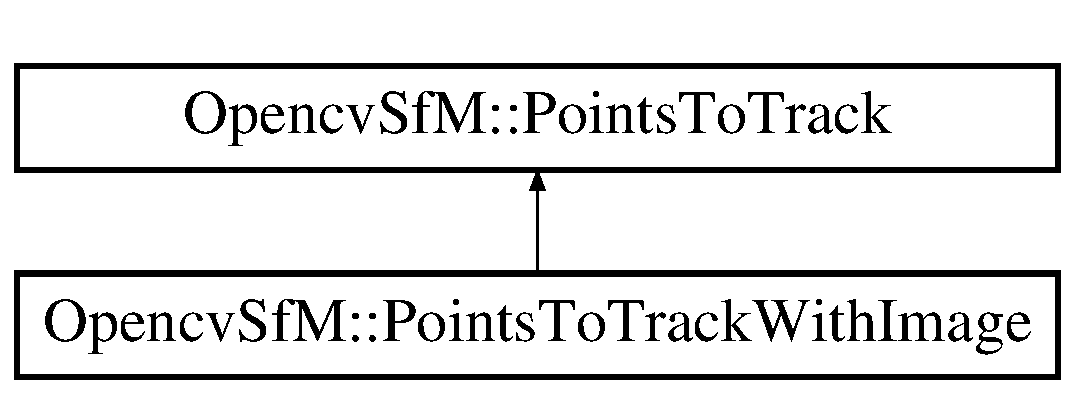
\includegraphics[height=2.000000cm]{class_opencv_sf_m_1_1_points_to_track}
\end{center}
\end{figure}
\subsection*{Public Member Functions}
\begin{DoxyCompactItemize}
\item 
\hyperlink{class_opencv_sf_m_1_1_points_to_track_a0974269063e5a7708e1b992480666f87}{PointsToTrack} (std::vector$<$ cv::KeyPoint $>$ keypoints=std::vector$<$ cv::KeyPoint $>$(0), cv::Mat descriptors=cv::Mat())
\item 
virtual \hyperlink{class_opencv_sf_m_1_1_points_to_track_a530e94d0c39358538d907e977263cae0}{$\sim$PointsToTrack} (void)
\item 
virtual int \hyperlink{class_opencv_sf_m_1_1_points_to_track_ab672d2d9b350500dde92f0d39c8c2a98}{computeKeypointsAndDesc} ()
\item 
virtual int \hyperlink{class_opencv_sf_m_1_1_points_to_track_ac7009164560dac1f4d3283c4bf1181a3}{computeKeypoints} ()
\item 
virtual void \hyperlink{class_opencv_sf_m_1_1_points_to_track_a1e5ef9b8da87d1b412c348ad813d0267}{computeDescriptors} ()
\item 
virtual void \hyperlink{class_opencv_sf_m_1_1_points_to_track_a6ac0b2e69bb0fa51af529ec395fd0df7}{addKeypoints} (std::vector$<$ cv::KeyPoint $>$ keypoints, cv::Mat descriptors=cv::Mat(), bool computeMissingDescriptor=false)
\item 
std::vector$<$ cv::KeyPoint $>$ \hyperlink{class_opencv_sf_m_1_1_points_to_track_ab646203ef4a8955b9540ffc5b78943d4}{getKeypoints} () const 
\item 
cv::Mat \hyperlink{class_opencv_sf_m_1_1_points_to_track_a4ca955b907dee279030559d255a4e151}{getDescriptors} () const 
\item 
void \hyperlink{class_opencv_sf_m_1_1_points_to_track_adda3cb43ad421e89b8ddfe24f1c30b30}{printPointsOnImage} (const cv::Mat \&image, cv::Mat \&outImg, const cv::Scalar \&color=cv::Scalar::all(-\/1), int flags=cv::DrawMatchesFlags::DEFAULT) const 
\item 
\hypertarget{class_opencv_sf_m_1_1_points_to_track_a2a3e9cb24add788e7c4970d248d789ba}{
void {\bfseries read} (const cv::FileNode \&fn)}
\label{class_opencv_sf_m_1_1_points_to_track_a2a3e9cb24add788e7c4970d248d789ba}

\item 
\hypertarget{class_opencv_sf_m_1_1_points_to_track_a4313423bb8db1700a7639fbfddb173b5}{
void {\bfseries write} (cv::FileStorage \&fs) const }
\label{class_opencv_sf_m_1_1_points_to_track_a4313423bb8db1700a7639fbfddb173b5}

\end{DoxyCompactItemize}
\subsection*{Protected Attributes}
\begin{DoxyCompactItemize}
\item 
\hypertarget{class_opencv_sf_m_1_1_points_to_track_a08c9523080571e71e30b11a2f8b9c6b9}{
std::vector$<$ cv::KeyPoint $>$ \hyperlink{class_opencv_sf_m_1_1_points_to_track_a08c9523080571e71e30b11a2f8b9c6b9}{keypoints\_\-}}
\label{class_opencv_sf_m_1_1_points_to_track_a08c9523080571e71e30b11a2f8b9c6b9}

\begin{DoxyCompactList}\small\item\em This attribute will store points coordinates and sometimes orientation and size. \end{DoxyCompactList}\item 
\hypertarget{class_opencv_sf_m_1_1_points_to_track_adcbf3783bdf4a2a1d3e10c4b74224899}{
cv::Mat \hyperlink{class_opencv_sf_m_1_1_points_to_track_adcbf3783bdf4a2a1d3e10c4b74224899}{descriptors\_\-}}
\label{class_opencv_sf_m_1_1_points_to_track_adcbf3783bdf4a2a1d3e10c4b74224899}

\begin{DoxyCompactList}\small\item\em this attribute will store descritors for each points in a matrix with size (n$\ast$m), where n is the number of points and m is the desciptor size. \end{DoxyCompactList}\end{DoxyCompactItemize}


\subsection{Detailed Description}
This class can be used to store informations about points and features. This is an abstract class: you can't use it directly. Use for instance PointsToTrackSIFT. 

To create a structure from motion, most methods use points to compute the structure. This class focus on the first task in SfM: find points in image which are easy to track... When available, a feature vector for each points is very helpful: the matching will be easier. 

Definition at line 18 of file PointsToTrack.h.



\subsection{Constructor \& Destructor Documentation}
\hypertarget{class_opencv_sf_m_1_1_points_to_track_a0974269063e5a7708e1b992480666f87}{
\index{OpencvSfM::PointsToTrack@{OpencvSfM::PointsToTrack}!PointsToTrack@{PointsToTrack}}
\index{PointsToTrack@{PointsToTrack}!OpencvSfM::PointsToTrack@{OpencvSfM::PointsToTrack}}
\subsubsection[{PointsToTrack}]{\setlength{\rightskip}{0pt plus 5cm}OpencvSfM::PointsToTrack::PointsToTrack (
\begin{DoxyParamCaption}
\item[{std::vector$<$ cv::KeyPoint $>$}]{keypoints = {\ttfamily std::vector$<$cv::KeyPoint$>$(0)}, }
\item[{cv::Mat}]{descriptors = {\ttfamily cv::Mat()}}
\end{DoxyParamCaption}
)}}
\label{class_opencv_sf_m_1_1_points_to_track_a0974269063e5a7708e1b992480666f87}
this constructor create an object with available information... 
\begin{DoxyParams}{Parameters}
{\em keypoints} & the points we will try to track... \\
\hline
{\em descriptors} & the feature vector for each points... \\
\hline
\end{DoxyParams}


Definition at line 12 of file PointsToTrack.cpp.

\hypertarget{class_opencv_sf_m_1_1_points_to_track_a530e94d0c39358538d907e977263cae0}{
\index{OpencvSfM::PointsToTrack@{OpencvSfM::PointsToTrack}!$\sim$PointsToTrack@{$\sim$PointsToTrack}}
\index{$\sim$PointsToTrack@{$\sim$PointsToTrack}!OpencvSfM::PointsToTrack@{OpencvSfM::PointsToTrack}}
\subsubsection[{$\sim$PointsToTrack}]{\setlength{\rightskip}{0pt plus 5cm}OpencvSfM::PointsToTrack::$\sim$PointsToTrack (
\begin{DoxyParamCaption}
\item[{void}]{}
\end{DoxyParamCaption}
)\hspace{0.3cm}{\ttfamily  \mbox{[}virtual\mbox{]}}}}
\label{class_opencv_sf_m_1_1_points_to_track_a530e94d0c39358538d907e977263cae0}
Destructor : delete points and features vectors 

Definition at line 17 of file PointsToTrack.cpp.



\subsection{Member Function Documentation}
\hypertarget{class_opencv_sf_m_1_1_points_to_track_a6ac0b2e69bb0fa51af529ec395fd0df7}{
\index{OpencvSfM::PointsToTrack@{OpencvSfM::PointsToTrack}!addKeypoints@{addKeypoints}}
\index{addKeypoints@{addKeypoints}!OpencvSfM::PointsToTrack@{OpencvSfM::PointsToTrack}}
\subsubsection[{addKeypoints}]{\setlength{\rightskip}{0pt plus 5cm}void OpencvSfM::PointsToTrack::addKeypoints (
\begin{DoxyParamCaption}
\item[{std::vector$<$ cv::KeyPoint $>$}]{keypoints, }
\item[{cv::Mat}]{descriptors = {\ttfamily cv::Mat()}, }
\item[{bool}]{computeMissingDescriptor = {\ttfamily false}}
\end{DoxyParamCaption}
)\hspace{0.3cm}{\ttfamily  \mbox{[}virtual\mbox{]}}}}
\label{class_opencv_sf_m_1_1_points_to_track_a6ac0b2e69bb0fa51af529ec395fd0df7}
This method is used to add Keypoints... 
\begin{DoxyParams}{Parameters}
{\em keypoints} & Keypoints to add \\
\hline
{\em descriptors} & of points, if any \\
\hline
{\em computeMissingDescriptor} & if true, the missing descriptors are computed. \\
\hline
\end{DoxyParams}


Definition at line 41 of file PointsToTrack.cpp.

\hypertarget{class_opencv_sf_m_1_1_points_to_track_a1e5ef9b8da87d1b412c348ad813d0267}{
\index{OpencvSfM::PointsToTrack@{OpencvSfM::PointsToTrack}!computeDescriptors@{computeDescriptors}}
\index{computeDescriptors@{computeDescriptors}!OpencvSfM::PointsToTrack@{OpencvSfM::PointsToTrack}}
\subsubsection[{computeDescriptors}]{\setlength{\rightskip}{0pt plus 5cm}void OpencvSfM::PointsToTrack::computeDescriptors (
\begin{DoxyParamCaption}
{}
\end{DoxyParamCaption}
)\hspace{0.3cm}{\ttfamily  \mbox{[}virtual\mbox{]}}}}
\label{class_opencv_sf_m_1_1_points_to_track_a1e5ef9b8da87d1b412c348ad813d0267}
This method is used to compute only descriptors... 

Reimplemented in \hyperlink{class_opencv_sf_m_1_1_points_to_track_with_image_aee97104c9c66601e5c51237717cb2522}{OpencvSfM::PointsToTrackWithImage}.



Definition at line 37 of file PointsToTrack.cpp.



Referenced by addKeypoints(), and computeKeypointsAndDesc().

\hypertarget{class_opencv_sf_m_1_1_points_to_track_ac7009164560dac1f4d3283c4bf1181a3}{
\index{OpencvSfM::PointsToTrack@{OpencvSfM::PointsToTrack}!computeKeypoints@{computeKeypoints}}
\index{computeKeypoints@{computeKeypoints}!OpencvSfM::PointsToTrack@{OpencvSfM::PointsToTrack}}
\subsubsection[{computeKeypoints}]{\setlength{\rightskip}{0pt plus 5cm}int OpencvSfM::PointsToTrack::computeKeypoints (
\begin{DoxyParamCaption}
{}
\end{DoxyParamCaption}
)\hspace{0.3cm}{\ttfamily  \mbox{[}virtual\mbox{]}}}}
\label{class_opencv_sf_m_1_1_points_to_track_ac7009164560dac1f4d3283c4bf1181a3}
This method is used to compute only Keypoints... \begin{DoxyReturn}{Returns}
the number of points 
\end{DoxyReturn}


Reimplemented in \hyperlink{class_opencv_sf_m_1_1_points_to_track_with_image_a4fba046ec6498fcea5b38253d19b80f9}{OpencvSfM::PointsToTrackWithImage}.



Definition at line 31 of file PointsToTrack.cpp.



Referenced by computeKeypointsAndDesc().

\hypertarget{class_opencv_sf_m_1_1_points_to_track_ab672d2d9b350500dde92f0d39c8c2a98}{
\index{OpencvSfM::PointsToTrack@{OpencvSfM::PointsToTrack}!computeKeypointsAndDesc@{computeKeypointsAndDesc}}
\index{computeKeypointsAndDesc@{computeKeypointsAndDesc}!OpencvSfM::PointsToTrack@{OpencvSfM::PointsToTrack}}
\subsubsection[{computeKeypointsAndDesc}]{\setlength{\rightskip}{0pt plus 5cm}int OpencvSfM::PointsToTrack::computeKeypointsAndDesc (
\begin{DoxyParamCaption}
{}
\end{DoxyParamCaption}
)\hspace{0.3cm}{\ttfamily  \mbox{[}virtual\mbox{]}}}}
\label{class_opencv_sf_m_1_1_points_to_track_ab672d2d9b350500dde92f0d39c8c2a98}
This method is used to compute both Keypoints and descriptors... \begin{DoxyReturn}{Returns}
the number of points 
\end{DoxyReturn}


Definition at line 23 of file PointsToTrack.cpp.

\hypertarget{class_opencv_sf_m_1_1_points_to_track_a4ca955b907dee279030559d255a4e151}{
\index{OpencvSfM::PointsToTrack@{OpencvSfM::PointsToTrack}!getDescriptors@{getDescriptors}}
\index{getDescriptors@{getDescriptors}!OpencvSfM::PointsToTrack@{OpencvSfM::PointsToTrack}}
\subsubsection[{getDescriptors}]{\setlength{\rightskip}{0pt plus 5cm}cv::Mat OpencvSfM::PointsToTrack::getDescriptors (
\begin{DoxyParamCaption}
{}
\end{DoxyParamCaption}
) const\hspace{0.3cm}{\ttfamily  \mbox{[}inline\mbox{]}}}}
\label{class_opencv_sf_m_1_1_points_to_track_a4ca955b907dee279030559d255a4e151}
this method return the descritors for each points in a matrix with size (n$\ast$m), where n is the number of points and m is the desciptor size. \begin{DoxyReturn}{Returns}
descritors for each points in a matrix with size (n$\ast$m), where n is the number of points and m is the desciptor size. 
\end{DoxyReturn}


Definition at line 65 of file PointsToTrack.h.

\hypertarget{class_opencv_sf_m_1_1_points_to_track_ab646203ef4a8955b9540ffc5b78943d4}{
\index{OpencvSfM::PointsToTrack@{OpencvSfM::PointsToTrack}!getKeypoints@{getKeypoints}}
\index{getKeypoints@{getKeypoints}!OpencvSfM::PointsToTrack@{OpencvSfM::PointsToTrack}}
\subsubsection[{getKeypoints}]{\setlength{\rightskip}{0pt plus 5cm}std::vector$<$cv::KeyPoint$>$ OpencvSfM::PointsToTrack::getKeypoints (
\begin{DoxyParamCaption}
{}
\end{DoxyParamCaption}
) const\hspace{0.3cm}{\ttfamily  \mbox{[}inline\mbox{]}}}}
\label{class_opencv_sf_m_1_1_points_to_track_ab646203ef4a8955b9540ffc5b78943d4}
this method return the points coordinates and sometimes orientation and size \begin{DoxyReturn}{Returns}
points coordinates and sometimes orientation and size 
\end{DoxyReturn}


Definition at line 60 of file PointsToTrack.h.

\hypertarget{class_opencv_sf_m_1_1_points_to_track_adda3cb43ad421e89b8ddfe24f1c30b30}{
\index{OpencvSfM::PointsToTrack@{OpencvSfM::PointsToTrack}!printPointsOnImage@{printPointsOnImage}}
\index{printPointsOnImage@{printPointsOnImage}!OpencvSfM::PointsToTrack@{OpencvSfM::PointsToTrack}}
\subsubsection[{printPointsOnImage}]{\setlength{\rightskip}{0pt plus 5cm}void OpencvSfM::PointsToTrack::printPointsOnImage (
\begin{DoxyParamCaption}
\item[{const cv::Mat \&}]{image, }
\item[{cv::Mat \&}]{outImg, }
\item[{const cv::Scalar \&}]{color = {\ttfamily cv::Scalar::all(-\/1)}, }
\item[{int}]{flags = {\ttfamily cv::DrawMatchesFlags::DEFAULT}}
\end{DoxyParamCaption}
) const}}
\label{class_opencv_sf_m_1_1_points_to_track_adda3cb43ad421e89b8ddfe24f1c30b30}
To show the points on image, use this function to draw points on it. 
\begin{DoxyParams}{Parameters}
{\em image} & Source image. \\
\hline
{\em outImg} & Output image. Its content depends on flags value what is drawn in output image. See possible flags bit values. \\
\hline
{\em color} & Color of keypoints \\
\hline
{\em flags} & Possible flags bit values is defined by DrawMatchesFlags (see \href{http://opencv.willowgarage.com/documentation/cpp/features2d_drawing_function_of_keypoints_and_matches.html#cv-drawmatches}{\tt http://opencv.willowgarage.com/documentation/cpp/features2d\_\-drawing\_\-function\_\-of\_\-keypoints\_\-and\_\-matches.html\#cv-\/drawmatches}) \\
\hline
\end{DoxyParams}


Definition at line 64 of file PointsToTrack.cpp.



The documentation for this class was generated from the following files:\begin{DoxyCompactItemize}
\item 
D:/Travail/These/Determination caracteristiques camera/GSoC/SfM/src/PointsToTrack.h\item 
D:/Travail/These/Determination caracteristiques camera/GSoC/SfM/src/PointsToTrack.cpp\end{DoxyCompactItemize}

\hypertarget{class_opencv_sf_m_1_1_points_to_track_with_image}{
\section{OpencvSfM::PointsToTrackWithImage Class Reference}
\label{class_opencv_sf_m_1_1_points_to_track_with_image}\index{OpencvSfM::PointsToTrackWithImage@{OpencvSfM::PointsToTrackWithImage}}
}


This class can be used to find points and features in pictures using SIFT detector.  




{\ttfamily \#include $<$PointsToTrackWithImage.h$>$}

Inheritance diagram for OpencvSfM::PointsToTrackWithImage:\begin{figure}[H]
\begin{center}
\leavevmode
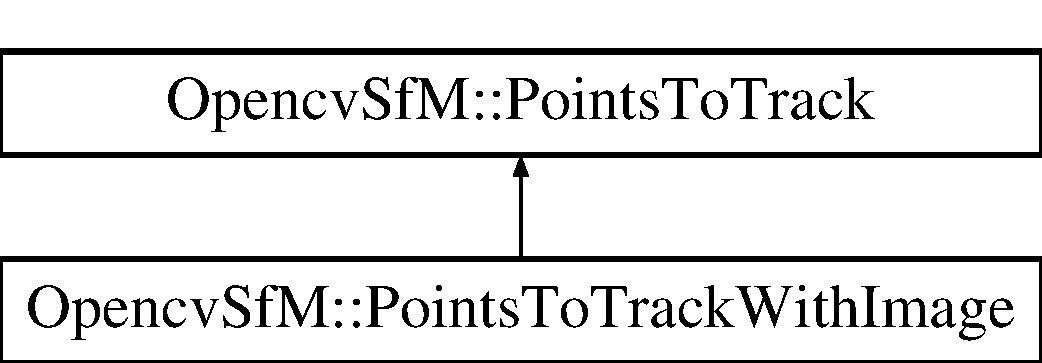
\includegraphics[height=2.000000cm]{class_opencv_sf_m_1_1_points_to_track_with_image}
\end{center}
\end{figure}
\subsection*{Public Member Functions}
\begin{DoxyCompactItemize}
\item 
\hyperlink{class_opencv_sf_m_1_1_points_to_track_with_image_a16b5fffabd61a2e728c1d677307d221e}{PointsToTrackWithImage} (cv::Mat imageToAnalyse, cv::Mat maskOfAnalyse, cv::Ptr$<$ cv::FeatureDetector $>$ feature\_\-detector=0, cv::Ptr$<$ cv::DescriptorExtractor $>$ descriptor\_\-detector=0)
\item 
\hyperlink{class_opencv_sf_m_1_1_points_to_track_with_image_a617869848cca4ee8f7933b203eaf8638}{PointsToTrackWithImage} (cv::Mat imageToAnalyse, cv::Mat maskOfAnalyse, std::string feature\_\-detector, std::string descriptor\_\-detector=\char`\"{}SIFT\char`\"{})
\item 
void \hyperlink{class_opencv_sf_m_1_1_points_to_track_with_image_a08e85521d6884eec1d113dd81354502f}{setFeatureDetector} (cv::Ptr$<$ cv::FeatureDetector $>$ feature\_\-detector)
\item 
void \hyperlink{class_opencv_sf_m_1_1_points_to_track_with_image_a3438e554c9ef0d807ccad6799209bb50}{setDescriptorExtractor} (cv::Ptr$<$ cv::DescriptorExtractor $>$ descriptor\_\-detector)
\item 
int \hyperlink{class_opencv_sf_m_1_1_points_to_track_with_image_a4fba046ec6498fcea5b38253d19b80f9}{computeKeypoints} ()
\item 
void \hyperlink{class_opencv_sf_m_1_1_points_to_track_with_image_aee97104c9c66601e5c51237717cb2522}{computeDescriptors} ()
\end{DoxyCompactItemize}
\subsection*{Protected Attributes}
\begin{DoxyCompactItemize}
\item 
\hypertarget{class_opencv_sf_m_1_1_points_to_track_with_image_a22779db7344fed472cebc4a00ecef631}{
cv::Ptr$<$ cv::FeatureDetector $>$ \hyperlink{class_opencv_sf_m_1_1_points_to_track_with_image_a22779db7344fed472cebc4a00ecef631}{feature\_\-detector\_\-}}
\label{class_opencv_sf_m_1_1_points_to_track_with_image_a22779db7344fed472cebc4a00ecef631}

\begin{DoxyCompactList}\small\item\em class which will find the points \end{DoxyCompactList}\item 
\hypertarget{class_opencv_sf_m_1_1_points_to_track_with_image_ac43985b39b4b99ffff25926f1e9ece66}{
cv::Ptr$<$ cv::DescriptorExtractor $>$ \hyperlink{class_opencv_sf_m_1_1_points_to_track_with_image_ac43985b39b4b99ffff25926f1e9ece66}{descriptor\_\-detector\_\-}}
\label{class_opencv_sf_m_1_1_points_to_track_with_image_ac43985b39b4b99ffff25926f1e9ece66}

\begin{DoxyCompactList}\small\item\em class which will compute the descriptors \end{DoxyCompactList}\item 
\hypertarget{class_opencv_sf_m_1_1_points_to_track_with_image_adccc33e14b09ecbe0d5963b405e58d48}{
cv::Mat \hyperlink{class_opencv_sf_m_1_1_points_to_track_with_image_adccc33e14b09ecbe0d5963b405e58d48}{imageToAnalyse\_\-}}
\label{class_opencv_sf_m_1_1_points_to_track_with_image_adccc33e14b09ecbe0d5963b405e58d48}

\begin{DoxyCompactList}\small\item\em Picture from where points are detected. \end{DoxyCompactList}\item 
\hypertarget{class_opencv_sf_m_1_1_points_to_track_with_image_a4fe39d059ba8a892abe3a1d998626806}{
cv::Mat \hyperlink{class_opencv_sf_m_1_1_points_to_track_with_image_a4fe39d059ba8a892abe3a1d998626806}{maskOfAnalyse\_\-}}
\label{class_opencv_sf_m_1_1_points_to_track_with_image_a4fe39d059ba8a892abe3a1d998626806}

\begin{DoxyCompactList}\small\item\em Mask of analyse. Everything out of this mask is ignored. \end{DoxyCompactList}\end{DoxyCompactItemize}


\subsection{Detailed Description}
This class can be used to find points and features in pictures using SIFT detector. 

To create a structure from motion, most methods use points to compute the structure. This class focus on the first task in SfM: find points in image which are easy to track... When available, a feature vector for each points is very helpful: the matching will be easier. 

Definition at line 14 of file PointsToTrackWithImage.h.



\subsection{Constructor \& Destructor Documentation}
\hypertarget{class_opencv_sf_m_1_1_points_to_track_with_image_a16b5fffabd61a2e728c1d677307d221e}{
\index{OpencvSfM::PointsToTrackWithImage@{OpencvSfM::PointsToTrackWithImage}!PointsToTrackWithImage@{PointsToTrackWithImage}}
\index{PointsToTrackWithImage@{PointsToTrackWithImage}!OpencvSfM::PointsToTrackWithImage@{OpencvSfM::PointsToTrackWithImage}}
\subsubsection[{PointsToTrackWithImage}]{\setlength{\rightskip}{0pt plus 5cm}OpencvSfM::PointsToTrackWithImage::PointsToTrackWithImage (
\begin{DoxyParamCaption}
\item[{cv::Mat}]{imageToAnalyse, }
\item[{cv::Mat}]{maskOfAnalyse, }
\item[{cv::Ptr$<$ cv::FeatureDetector $>$}]{feature\_\-detector = {\ttfamily 0}, }
\item[{cv::Ptr$<$ cv::DescriptorExtractor $>$}]{descriptor\_\-detector = {\ttfamily 0}}
\end{DoxyParamCaption}
)}}
\label{class_opencv_sf_m_1_1_points_to_track_with_image_a16b5fffabd61a2e728c1d677307d221e}
First constructor used to create a list of points to track using a feature and a descriptor algorithm. 
\begin{DoxyParams}{Parameters}
{\em imageToAnalyse} & Image to use for keypoints and features search \\
\hline
{\em maskOfAnalyse} & Mask used to hide part of image \\
\hline
{\em feature\_\-detector} & Algorithm to use for features detection (see \href{http://opencv.willowgarage.com/documentation/cpp/common_interfaces_for_feature_detection_and_descriptor_extraction.html#featuredetector}{\tt http://opencv.willowgarage.com/documentation/cpp/common\_\-interfaces\_\-for\_\-feature\_\-detection\_\-and\_\-descriptor\_\-extraction.html\#featuredetector}) \\
\hline
{\em descriptor\_\-detector} & Algorithm to use for descriptors detection (see \href{http://opencv.willowgarage.com/documentation/cpp/common_interfaces_for_feature_detection_and_descriptor_extraction.html#descriptorextractor}{\tt http://opencv.willowgarage.com/documentation/cpp/common\_\-interfaces\_\-for\_\-feature\_\-detection\_\-and\_\-descriptor\_\-extraction.html\#descriptorextractor}) \\
\hline
\end{DoxyParams}
\hypertarget{class_opencv_sf_m_1_1_points_to_track_with_image_a617869848cca4ee8f7933b203eaf8638}{
\index{OpencvSfM::PointsToTrackWithImage@{OpencvSfM::PointsToTrackWithImage}!PointsToTrackWithImage@{PointsToTrackWithImage}}
\index{PointsToTrackWithImage@{PointsToTrackWithImage}!OpencvSfM::PointsToTrackWithImage@{OpencvSfM::PointsToTrackWithImage}}
\subsubsection[{PointsToTrackWithImage}]{\setlength{\rightskip}{0pt plus 5cm}OpencvSfM::PointsToTrackWithImage::PointsToTrackWithImage (
\begin{DoxyParamCaption}
\item[{cv::Mat}]{imageToAnalyse, }
\item[{cv::Mat}]{maskOfAnalyse, }
\item[{std::string}]{feature\_\-detector, }
\item[{std::string}]{descriptor\_\-detector = {\ttfamily \char`\"{}SIFT\char`\"{}}}
\end{DoxyParamCaption}
)}}
\label{class_opencv_sf_m_1_1_points_to_track_with_image_a617869848cca4ee8f7933b203eaf8638}
Second constructor used to create a list of points to track using a feature and a descriptor algorithm. 
\begin{DoxyParams}{Parameters}
{\em imageToAnalyse} & Image to use for keypoints and features search \\
\hline
{\em maskOfAnalyse} & Mask used to hide part of image \\
\hline
{\em feature\_\-detector} & name of the algorithm to use for features detection (see \href{http://opencv.willowgarage.com/documentation/cpp/common_interfaces_for_feature_detection_and_descriptor_extraction.html#featuredetector}{\tt http://opencv.willowgarage.com/documentation/cpp/common\_\-interfaces\_\-for\_\-feature\_\-detection\_\-and\_\-descriptor\_\-extraction.html\#featuredetector}) \\
\hline
{\em descriptor\_\-detector} & name of the algorithm to use for descriptors detection (see \href{http://opencv.willowgarage.com/documentation/cpp/common_interfaces_for_feature_detection_and_descriptor_extraction.html#descriptorextractor}{\tt http://opencv.willowgarage.com/documentation/cpp/common\_\-interfaces\_\-for\_\-feature\_\-detection\_\-and\_\-descriptor\_\-extraction.html\#descriptorextractor}) \\
\hline
\end{DoxyParams}


\subsection{Member Function Documentation}
\hypertarget{class_opencv_sf_m_1_1_points_to_track_with_image_aee97104c9c66601e5c51237717cb2522}{
\index{OpencvSfM::PointsToTrackWithImage@{OpencvSfM::PointsToTrackWithImage}!computeDescriptors@{computeDescriptors}}
\index{computeDescriptors@{computeDescriptors}!OpencvSfM::PointsToTrackWithImage@{OpencvSfM::PointsToTrackWithImage}}
\subsubsection[{computeDescriptors}]{\setlength{\rightskip}{0pt plus 5cm}void OpencvSfM::PointsToTrackWithImage::computeDescriptors (
\begin{DoxyParamCaption}
{}
\end{DoxyParamCaption}
)\hspace{0.3cm}{\ttfamily  \mbox{[}virtual\mbox{]}}}}
\label{class_opencv_sf_m_1_1_points_to_track_with_image_aee97104c9c66601e5c51237717cb2522}
This method is used to compute only descriptors... 

Reimplemented from \hyperlink{class_opencv_sf_m_1_1_points_to_track_a1e5ef9b8da87d1b412c348ad813d0267}{OpencvSfM::PointsToTrack}.



Definition at line 45 of file PointsToTrackWithImage.cpp.

\hypertarget{class_opencv_sf_m_1_1_points_to_track_with_image_a4fba046ec6498fcea5b38253d19b80f9}{
\index{OpencvSfM::PointsToTrackWithImage@{OpencvSfM::PointsToTrackWithImage}!computeKeypoints@{computeKeypoints}}
\index{computeKeypoints@{computeKeypoints}!OpencvSfM::PointsToTrackWithImage@{OpencvSfM::PointsToTrackWithImage}}
\subsubsection[{computeKeypoints}]{\setlength{\rightskip}{0pt plus 5cm}int OpencvSfM::PointsToTrackWithImage::computeKeypoints (
\begin{DoxyParamCaption}
{}
\end{DoxyParamCaption}
)\hspace{0.3cm}{\ttfamily  \mbox{[}virtual\mbox{]}}}}
\label{class_opencv_sf_m_1_1_points_to_track_with_image_a4fba046ec6498fcea5b38253d19b80f9}
This method is used to compute only Keypoints... \begin{DoxyReturn}{Returns}
the number of points 
\end{DoxyReturn}


Reimplemented from \hyperlink{class_opencv_sf_m_1_1_points_to_track_ac7009164560dac1f4d3283c4bf1181a3}{OpencvSfM::PointsToTrack}.



Definition at line 39 of file PointsToTrackWithImage.cpp.

\hypertarget{class_opencv_sf_m_1_1_points_to_track_with_image_a3438e554c9ef0d807ccad6799209bb50}{
\index{OpencvSfM::PointsToTrackWithImage@{OpencvSfM::PointsToTrackWithImage}!setDescriptorExtractor@{setDescriptorExtractor}}
\index{setDescriptorExtractor@{setDescriptorExtractor}!OpencvSfM::PointsToTrackWithImage@{OpencvSfM::PointsToTrackWithImage}}
\subsubsection[{setDescriptorExtractor}]{\setlength{\rightskip}{0pt plus 5cm}void OpencvSfM::PointsToTrackWithImage::setDescriptorExtractor (
\begin{DoxyParamCaption}
\item[{cv::Ptr$<$ cv::DescriptorExtractor $>$}]{descriptor\_\-detector}
\end{DoxyParamCaption}
)}}
\label{class_opencv_sf_m_1_1_points_to_track_with_image_a3438e554c9ef0d807ccad6799209bb50}
Use this function to set the descriptor extractor. Can be useful to update parameters, for example! 
\begin{DoxyParams}{Parameters}
{\em descriptor\_\-detector} & new pointer of a descriptor extractor algorithm. \\
\hline
\end{DoxyParams}


Definition at line 28 of file PointsToTrackWithImage.cpp.

\hypertarget{class_opencv_sf_m_1_1_points_to_track_with_image_a08e85521d6884eec1d113dd81354502f}{
\index{OpencvSfM::PointsToTrackWithImage@{OpencvSfM::PointsToTrackWithImage}!setFeatureDetector@{setFeatureDetector}}
\index{setFeatureDetector@{setFeatureDetector}!OpencvSfM::PointsToTrackWithImage@{OpencvSfM::PointsToTrackWithImage}}
\subsubsection[{setFeatureDetector}]{\setlength{\rightskip}{0pt plus 5cm}void OpencvSfM::PointsToTrackWithImage::setFeatureDetector (
\begin{DoxyParamCaption}
\item[{cv::Ptr$<$ cv::FeatureDetector $>$}]{feature\_\-detector}
\end{DoxyParamCaption}
)}}
\label{class_opencv_sf_m_1_1_points_to_track_with_image_a08e85521d6884eec1d113dd81354502f}
Use this function to set the feature detector. Can be useful to update parameters, for example! 
\begin{DoxyParams}{Parameters}
{\em feature\_\-detector} & new pointer of a feature detector algorithm. \\
\hline
\end{DoxyParams}


Definition at line 23 of file PointsToTrackWithImage.cpp.



The documentation for this class was generated from the following files:\begin{DoxyCompactItemize}
\item 
src/PointsToTrackWithImage.h\item 
src/PointsToTrackWithImage.cpp\end{DoxyCompactItemize}

\printindex
\end{document}
